\documentclass[letterpaper,12pt]{article}
\usepackage{graphicx}
\usepackage[top=1.10in,right=1.2in,bottom=1.4in,left=1.2in]{geometry} 

\frenchspacing  % Removes extra spacing after period.

\usepackage{hyperref}

\usepackage{natbib}
%\usepackage{times}

\usepackage{amsmath}
%\usepackage{hyperref}

\usepackage{color}

\usepackage{pa}

\newcommand{\proglang}{\texttt}
\newcommand{\pkg}{\texttt}


\title{EPC-interest for categorical data with an application to the Inglehart values ranking}
\date{}

\author{\;}

\usepackage{bm}
\newcommand\vm[1]{% Vector or matrix
\bm{\mathrm{#1}}} 

\newcommand{\av}{\vm{a}}
\newcommand{\vech}{\mathrm{vech}\,}
\newcommand{\vecs}{\mathrm{vec}\,}
\newcommand{\that}{\hat{\vm{\theta}}}
\newcommand{\A}{\vm{A}}
\newcommand{\g}{\vm{g}}
\newcommand{\J}{\vm{J}}
\newcommand{\Id}{\vm{I}}
\newcommand{\Ji}{\vm{J}^{-1}}
\newcommand{\PP}{\vm{P}}
\newcommand{\da}{\textrm{{\sc {EPC}}-interest}}

\usepackage{setspace}
\doublespacing

\begin{document}
\maketitle



\begin{abstract}
Social science is often concerned with comparing groups such as countries, regions, time periods, the genders, or ethnicities.
Because such substantive comparisons may be threatened when measurement parameters differ across the groups, it is common practice to test the hypothesis of exact equality of measurement parameters across groups:  ``measurement invariance testing''. However, not all measurement differences are substantively relevant. At the same time, it was recently shown that not all substantively relevant differences are necessarily detected by the current best practices of invariance testing. Therefore, it was recently suggested to detect the relevant set of violations of measurement invariance using sensitivity analysis. This approach, recently introduced in this journal, uses the ``EPC-interest'',  a measure of the change in the parameters of substantive interest due to violations of invariance. The EPC-interest was limited to continuous linear structural equation models and did not consider the impact of freeing several restrictions at the same time. However, categorical data are common in the social sciences and measurement invariance restrictions are typically highly correlated.

This paper therefore extends the ``EPC-interest'' to models with categorical observed and latent variables. Moreover, we explicitly consider freeing (potentially large) sets of equality restrictions simultaneously. The advantages of the extended EPC-interest are demonstrated using a 48 country analysis of ``materialism/postmaterialism'' values measured by three partial ranking tasks using multilevel latent class regression. Some corroboration for hypotheses on postmaterialism from the literature are found when employing the EPC-interest, while without its application some of the findings contradict these hypotheses.

The newly developed methods discussed in this paper have been implemented in commercial software for latent variable modeling. Program inputs and data for the examples discussed in this article are provided in the electronic appendix (\url{http://}).
\end{abstract}

\section{Introduction}

\noindent


The logic of measurement invariance testing is that groups may safely be compared when their measurement parameters are exactly equal: in that case, conclusions of substantive interest are uncontaminated by measurement differences. While this logic is sound, it does not follow that comparison is never warranted when measurement parameters are not exactly equal. Moreover, in practical applications exact equality is not often plausible. These observations have led to the concept of ``approximate'' measurement  invariance, in which a certain, ``small'' amount of non-invariance is permitted. 
%``Approximate'' has in the past been taken to correspond to model fit in terms of CFI, RMSEA and other relative fit measures, while more recently Bayesian priors on group differences and the alignment method were introduced. 
However, while these methods ensure that measurement differences are ``small'', even ``small'' measurement differences could, in principle, still contaminate the conclusions of interest. Conversely, those measurement differences allowed for may not necessarily affect the conclusions of interest. 



\section{EPC-interest}

\section{Data}
\section{Model}
\section{Results}

Latent Gold Choice 5.0.0.14157

LL = -418609.9616

Number of parameters (Npar)	63


\begin{table}
	\begin{tabular}{lrrrrrrrrrrr}
	\hline
		&&&&&\multicolumn{7}{c}{EPC-interest for non-invariance of...}\\
	&&&&&\multicolumn{3}{c}{Set main effects} && \multicolumn{3}{c}{Set $\times$ Class effects}\\
			\hline
		&&&&&\multicolumn{3}{c}{Set} && \multicolumn{3}{c}{Set}\\
\cline{6-8}\cline{10-12}
			&	&	Est.&	s.e.&	&	1  &	2  &	3  &&	  1&	2 &	3\\
				\hline
Class	1&	GDP&	-0.035&	(0.007)&	&	-0.013&	0.021&	-0.002&&	\textbf{0.073}&	\textbf{0.252}&	0.005\\
Class	2&	GDP&	-0.198&	(0.012)&	&	-0.018&	-0.035&	0.015&&	-0.163&	-0.058&	0.002\\
\\
Class	1&	Women&	0.013&	(0.001)&	&	-0.006&	0.002&	0.000&&	-0.003&	0.029&	0.002\\
Class	2&	Women&	-0.037&	(0.001)&	&	0.007&	-0.003&	0.002&&	-0.006&	-0.013&	0.002\\
	\hline
\end{tabular}
	\caption{\label{tab:epc-interest-model1}}
\end{table}

\begin{table}
	\begin{tabular}{lrrrrrrrrrrr}
	\hline
		&&&&&\multicolumn{7}{c}{EPC-interest for non-invariance of...}\\
	&&&&&\multicolumn{3}{c}{Set main effects} && \multicolumn{3}{c}{Set $\times$ Class effects}\\
			\hline
		&&&&&\multicolumn{3}{c}{Set} && \multicolumn{3}{c}{Set}\\
\cline{6-8}\cline{10-12}
			&	&	Est.&	s.e.&	&	1  &	2  &	3  &&	  1&	2 &	3\\
				\hline
Class 1&	GDP&	-0.127&	(0.008)&	&	-0.015&	-0.003&	0.002&&	&	&	0.097\\
Class 2&	GDP&	0.057&	(0.011)&	&	-0.043&	-0.013&	0.002&&	&	&	0.161\\
\\
Class 	1&	Women&	0.008&	(0.001)&	&	-0.002&	0.000&	0.002&	&&	&	0.001\\
Class 	2&	Women&	0.020&	(0.001)&	&	-0.007&	-0.001&	0.002&	&&	&	0.007\\
\hline
	\end{tabular}
	\caption{\label{tab:epc-interest-model2}}

\end{table}



\begin{table}\centering
	\begin{tabular}{llrrr}
	\hline
			&&	Class 1	&	Class 2	&	Class 3\\
			&Class label& ``Materialist'' & ``Postmater.'' & ``Mixed''\\
& Class size & 0.569 & 0.213 & 0.218\\
				\hline
\multicolumn{3}{l}{Set 1}\\
& 1. Economic growth	&	2.1102	&	0.4837	&	0.4156\\
& 2. Strong defense	&	-0.5285	&	-1.4984	&	-0.9249\\
& 3. More say	&	-0.5519	&	1.4683	&	0.4643\\
& 4. More beauty	&	-1.0298	&	-0.4536	&	0.0449\\
\multicolumn{3}{l}{Set 2}\\
& 1. Order in the nation	&	1.0016	&	-0.5898	&	0.0435\\
& 2. More say	&	-0.4592	&	0.6902	&	-0.2763\\
& 3. Rising prices	&	0.4281	&	-0.2269	&	0.3719\\
& 4. Freedom of speech	&	-0.9705	&	0.1266	&	-0.1390\\
\multicolumn{3}{l}{Set 3}\\
& 1. Stable economy	&	2.0086	&	0.0789	&	0.1715\\
& 2. Humane society	&	-0.7919	&	0.4450	&	-0.0943\\
& 3. Ideas	&	-1.1402	&	-0.0593	&	-0.4550\\
& 4. Fight crime	&	-0.0765	&	-0.4646	&	0.3778\\
	\hline
	\end{tabular}
	\caption{\label{tab:attribute-parameters}Attribute parameter estimates for the 
		final model.}

\end{table}


\begin{figure}
	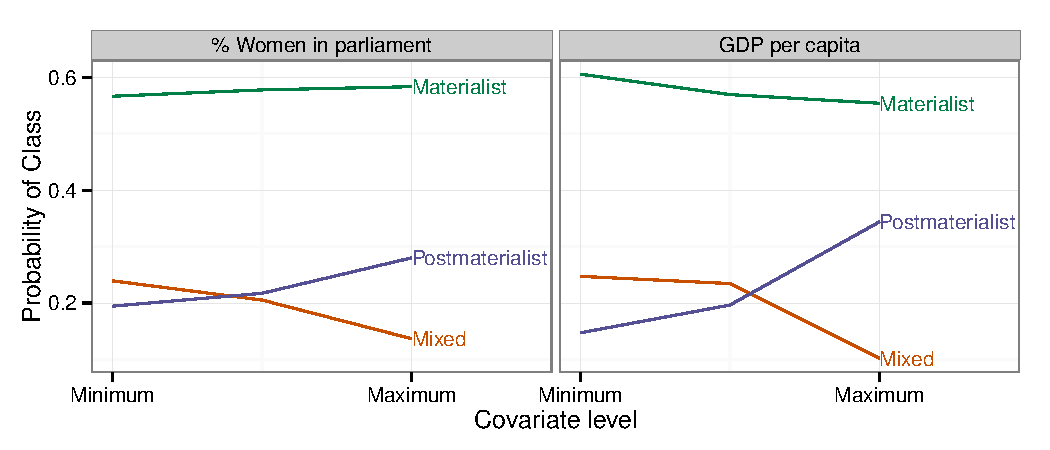
\includegraphics[width=\textwidth]{figures/covariates.pdf}
	\caption{\label{fig:covariates}Estimated probability of choosing each class as a function of the covariates of interest under the final model.}
\end{figure}

\begin{figure}
	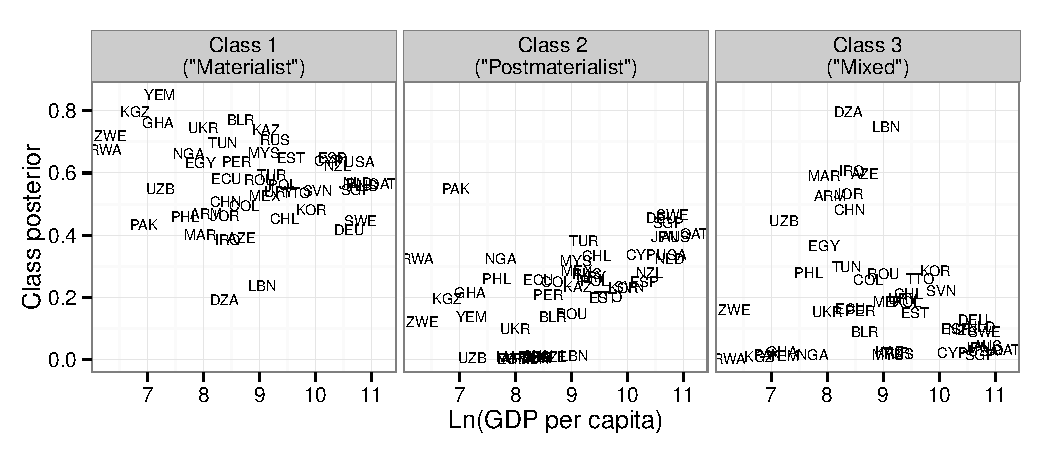
\includegraphics[width=\textwidth]{figures/gdp-posterior.pdf}
	
	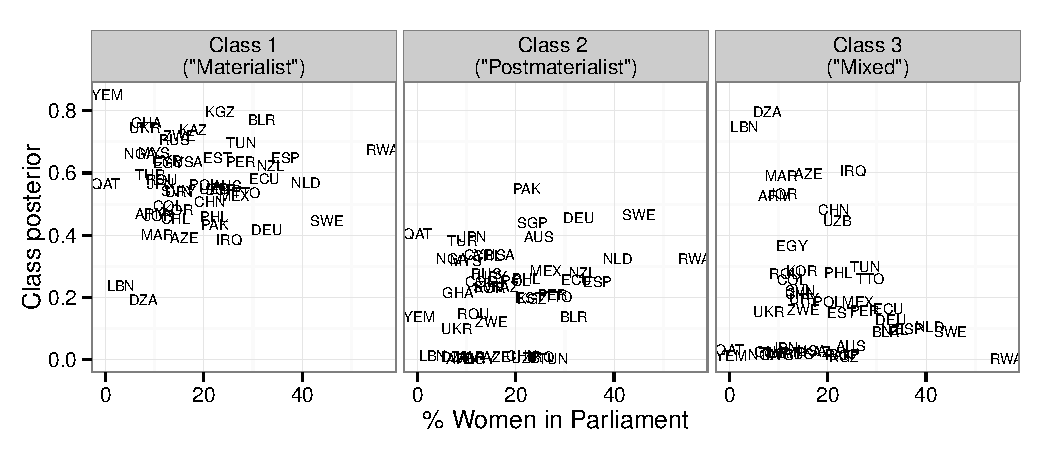
\includegraphics[width=\textwidth]{figures/women-posterior.pdf}

	\caption{\label{fig:posterior}}
\end{figure}

\begin{figure}
	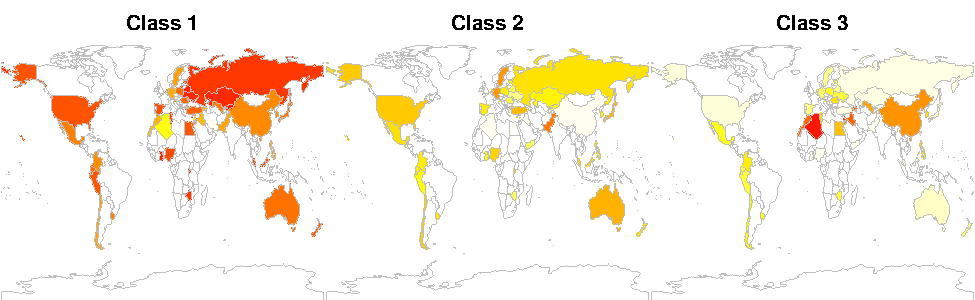
\includegraphics[width=\textwidth]{figures/maps.pdf}
	
	\caption{\label{fig:maps}}
\end{figure}

\section{Discussion}



\bibliographystyle{pa}
\bibliography{/Users/daob/Dropbox/Bibliography/quality}

\end{document}
